\documentclass{article}\usepackage[]{graphicx}\usepackage[]{color}
% maxwidth is the original width if it is less than linewidth
% otherwise use linewidth (to make sure the graphics do not exceed the margin)
\makeatletter
\def\maxwidth{ %
  \ifdim\Gin@nat@width>\linewidth
    \linewidth
  \else
    \Gin@nat@width
  \fi
}
\makeatother

\definecolor{fgcolor}{rgb}{0.345, 0.345, 0.345}
\newcommand{\hlnum}[1]{\textcolor[rgb]{0.686,0.059,0.569}{#1}}%
\newcommand{\hlstr}[1]{\textcolor[rgb]{0.192,0.494,0.8}{#1}}%
\newcommand{\hlcom}[1]{\textcolor[rgb]{0.678,0.584,0.686}{\textit{#1}}}%
\newcommand{\hlopt}[1]{\textcolor[rgb]{0,0,0}{#1}}%
\newcommand{\hlstd}[1]{\textcolor[rgb]{0.345,0.345,0.345}{#1}}%
\newcommand{\hlkwa}[1]{\textcolor[rgb]{0.161,0.373,0.58}{\textbf{#1}}}%
\newcommand{\hlkwb}[1]{\textcolor[rgb]{0.69,0.353,0.396}{#1}}%
\newcommand{\hlkwc}[1]{\textcolor[rgb]{0.333,0.667,0.333}{#1}}%
\newcommand{\hlkwd}[1]{\textcolor[rgb]{0.737,0.353,0.396}{\textbf{#1}}}%
\let\hlipl\hlkwb

\usepackage{framed}
\makeatletter
\newenvironment{kframe}{%
 \def\at@end@of@kframe{}%
 \ifinner\ifhmode%
  \def\at@end@of@kframe{\end{minipage}}%
  \begin{minipage}{\columnwidth}%
 \fi\fi%
 \def\FrameCommand##1{\hskip\@totalleftmargin \hskip-\fboxsep
 \colorbox{shadecolor}{##1}\hskip-\fboxsep
     % There is no \\@totalrightmargin, so:
     \hskip-\linewidth \hskip-\@totalleftmargin \hskip\columnwidth}%
 \MakeFramed {\advance\hsize-\width
   \@totalleftmargin\z@ \linewidth\hsize
   \@setminipage}}%
 {\par\unskip\endMakeFramed%
 \at@end@of@kframe}
\makeatother

\definecolor{shadecolor}{rgb}{.97, .97, .97}
\definecolor{messagecolor}{rgb}{0, 0, 0}
\definecolor{warningcolor}{rgb}{1, 0, 1}
\definecolor{errorcolor}{rgb}{1, 0, 0}
\newenvironment{knitrout}{}{} % an empty environment to be redefined in TeX

\usepackage{alltt}
\IfFileExists{upquote.sty}{\usepackage{upquote}}{}
\begin{document}



Load the necessary libraries:
\begin{knitrout}
\definecolor{shadecolor}{rgb}{0.969, 0.969, 0.969}\color{fgcolor}\begin{kframe}
\begin{alltt}
\hlkwd{library}\hlstd{(ggplot2)}
\hlkwd{library}\hlstd{(MCMCpack)}
\end{alltt}


{\ttfamily\noindent\color{warningcolor}{\#\# Warning: package 'MCMCpack' was built under R version 4.0.3}}

{\ttfamily\noindent\itshape\color{messagecolor}{\#\# Loading required package: coda}}

{\ttfamily\noindent\color{warningcolor}{\#\# Warning: package 'coda' was built under R version 4.0.3}}

{\ttfamily\noindent\itshape\color{messagecolor}{\#\# Loading required package: MASS}}

{\ttfamily\noindent\itshape\color{messagecolor}{\#\# \#\#\\\#\# \#\# Markov Chain Monte Carlo Package (MCMCpack)}}

{\ttfamily\noindent\itshape\color{messagecolor}{\#\# \#\# Copyright (C) 2003-2021 Andrew D. Martin, Kevin M. Quinn, and Jong Hee Park}}

{\ttfamily\noindent\itshape\color{messagecolor}{\#\# \#\#\\\#\# \#\# Support provided by the U.S. National Science Foundation}}

{\ttfamily\noindent\itshape\color{messagecolor}{\#\# \#\# (Grants SES-0350646 and SES-0350613)\\\#\# \#\#}}\begin{alltt}
\hlkwd{library}\hlstd{(gridExtra)}
\hlkwd{library}\hlstd{(Matrix)}
\end{alltt}
\end{kframe}
\end{knitrout}

\begin{knitrout}
\definecolor{shadecolor}{rgb}{0.969, 0.969, 0.969}\color{fgcolor}\begin{kframe}
\begin{alltt}
\hlcom{##function which calculates heterozygosity for admixture for given gamma }
\hlcom{##and allele frequencies}
\hlstd{Hadm} \hlkwb{<-} \hlkwa{function}\hlstd{(}\hlkwc{gamma}\hlstd{,} \hlkwc{P}\hlstd{)}
\hlstd{\{}
  \hlstd{K} \hlkwb{<-} \hlkwd{length}\hlstd{(gamma)}
  \hlstd{J} \hlkwb{<-} \hlkwd{nrow}\hlstd{(P)}

  \hlstd{pBar} \hlkwb{<-} \hlkwd{rep}\hlstd{(}\hlnum{0}\hlstd{, J)}

  \hlkwa{for}\hlstd{(k} \hlkwa{in} \hlnum{1}\hlopt{:}\hlstd{K)}
  \hlstd{\{}
    \hlstd{pBar} \hlkwb{<-} \hlstd{pBar} \hlopt{+} \hlstd{gamma[k]}\hlopt{*}\hlstd{P[,k]}
  \hlstd{\}}

  \hlcom{##pBar <- rowSums(gamma*P) ##.Internal(rowSums(gamma*P, J, K, na.rm=TRUE))}
  \hlnum{1} \hlopt{-} \hlkwd{sum}\hlstd{(pBar}\hlopt{^}\hlnum{2}\hlstd{)}
\hlstd{\}}
\end{alltt}
\end{kframe}
\end{knitrout}

\section{Do simulations!}

Note that the code below only does 1,000 simulations, as opposed to 50,000, as in the paper. Performing 50,000 simulations would probably overwhelm local computing resources and can be done via parallel implementation. As a result, the figure is not quite as smooth as the one in the paper, though the general trend is the same.
Increasing the number of simulations would increase the smoothness.

\begin{knitrout}
\definecolor{shadecolor}{rgb}{0.969, 0.969, 0.969}\color{fgcolor}\begin{kframe}
\begin{alltt}
\hlkwd{set.seed}\hlstd{(}\hlnum{231883}\hlstd{)}

\hlstd{nrSims} \hlkwb{<-} \hlnum{1000}

\hlcom{##save fraction of times Hadm is bigger than H1, ..., HK}
\hlstd{HadmBiggerMax} \hlkwb{<-} \hlkwd{expand.grid}\hlstd{(}\hlkwc{J} \hlstd{=} \hlnum{2}\hlopt{:}\hlnum{30}\hlstd{,} \hlkwc{K} \hlstd{=} \hlnum{2}\hlopt{:}\hlnum{5}\hlstd{,} \hlkwc{HadmBigger}\hlstd{=}\hlnum{0}\hlstd{)}

\hlstd{alphaBar} \hlkwb{<-} \hlnum{1}

\hlkwd{dim}\hlstd{(HadmBiggerMax)}
\end{alltt}
\begin{verbatim}
## [1] 116   3
\end{verbatim}
\begin{alltt}
\hlkwa{for}\hlstd{(i} \hlkwa{in} \hlnum{1}\hlopt{:}\hlkwd{nrow}\hlstd{(HadmBiggerMax))}
\hlstd{\{}
  \hlkwa{if}\hlstd{(i} \hlopt \hlnum{5} \hlopt{==} \hlnum{0}\hlstd{)}
  \hlstd{\{}
    \hlkwd{print}\hlstd{(}\hlkwd{c}\hlstd{(i,} \hlkwd{date}\hlstd{()))}
  \hlstd{\}}

  \hlstd{J} \hlkwb{<-} \hlstd{HadmBiggerMax[i,} \hlnum{1}\hlstd{]}
  \hlstd{K} \hlkwb{<-} \hlstd{HadmBiggerMax[i,} \hlnum{2}\hlstd{]}

  \hlkwa{for}\hlstd{(sim} \hlkwa{in} \hlnum{1}\hlopt{:}\hlstd{nrSims)}
  \hlstd{\{}
    \hlcom{##generate some allele frequencies}
    \hlstd{P} \hlkwb{<-} \hlkwd{t.default}\hlstd{(}\hlkwd{rdirichlet}\hlstd{(K,} \hlkwd{rep}\hlstd{(alphaBar, J)))}

    \hlcom{##generate some admixture fractions}
    \hlstd{gamma} \hlkwb{<-} \hlkwd{rdirichlet}\hlstd{(}\hlnum{1}\hlstd{,} \hlkwd{rep}\hlstd{(alphaBar, K))}

    \hlcom{##calculate H1, ..., HK}
    \hlstd{Hfounders} \hlkwb{<-} \hlkwd{rep}\hlstd{(}\hlnum{NA}\hlstd{, K)}
    \hlkwa{for}\hlstd{(k} \hlkwa{in} \hlnum{1}\hlopt{:}\hlstd{K)}
    \hlstd{\{}
      \hlcom{##e.k <- rep(0, K)}
      \hlcom{##e.k[k] <- 1}
      \hlstd{Hfounders[k]} \hlkwb{<-} \hlnum{1}\hlopt{-}\hlkwd{sum}\hlstd{(P[,k]}\hlopt{^}\hlnum{2}\hlstd{)}\hlcom{##Hadm(gamma=e.k, P=P)}
    \hlstd{\}}
    \hlcom{##calculate Hadm}
    \hlstd{Hadm.curr} \hlkwb{<-} \hlkwd{Hadm}\hlstd{(}\hlkwc{gamma}\hlstd{=gamma,} \hlkwc{P}\hlstd{=P)}

    \hlkwa{if}\hlstd{(}\hlkwd{sum}\hlstd{(Hadm.curr} \hlopt{>} \hlstd{Hfounders)} \hlopt{==} \hlstd{K)}
    \hlstd{\{}
      \hlstd{HadmBiggerMax[i,} \hlnum{3}\hlstd{]} \hlkwb{<-} \hlstd{HadmBiggerMax[i,} \hlnum{3}\hlstd{]} \hlopt{+} \hlnum{1}
    \hlstd{\}}
  \hlstd{\}}
\hlstd{\}}
\end{alltt}
\begin{verbatim}
## [1] "5"                        "Tue Jan 05 14:24:04 2021"
## [1] "10"                       "Tue Jan 05 14:24:05 2021"
## [1] "15"                       "Tue Jan 05 14:24:06 2021"
## [1] "20"                       "Tue Jan 05 14:24:07 2021"
## [1] "25"                       "Tue Jan 05 14:24:07 2021"
## [1] "30"                       "Tue Jan 05 14:24:08 2021"
## [1] "35"                       "Tue Jan 05 14:24:08 2021"
## [1] "40"                       "Tue Jan 05 14:24:09 2021"
## [1] "45"                       "Tue Jan 05 14:24:09 2021"
## [1] "50"                       "Tue Jan 05 14:24:09 2021"
## [1] "55"                       "Tue Jan 05 14:24:10 2021"
## [1] "60"                       "Tue Jan 05 14:24:10 2021"
## [1] "65"                       "Tue Jan 05 14:24:11 2021"
## [1] "70"                       "Tue Jan 05 14:24:11 2021"
## [1] "75"                       "Tue Jan 05 14:24:11 2021"
## [1] "80"                       "Tue Jan 05 14:24:12 2021"
## [1] "85"                       "Tue Jan 05 14:24:12 2021"
## [1] "90"                       "Tue Jan 05 14:24:13 2021"
## [1] "95"                       "Tue Jan 05 14:24:13 2021"
## [1] "100"                      "Tue Jan 05 14:24:14 2021"
## [1] "105"                      "Tue Jan 05 14:24:14 2021"
## [1] "110"                      "Tue Jan 05 14:24:15 2021"
## [1] "115"                      "Tue Jan 05 14:24:15 2021"
\end{verbatim}
\begin{alltt}
\hlkwd{range}\hlstd{(HadmBiggerMax[,} \hlnum{3}\hlstd{])}
\end{alltt}
\begin{verbatim}
## [1] 290 961
\end{verbatim}
\begin{alltt}
\hlstd{HadmBiggerMax[,} \hlnum{3}\hlstd{]} \hlkwb{<-} \hlstd{HadmBiggerMax[,} \hlnum{3}\hlstd{]}\hlopt{/}\hlstd{nrSims}
\hlkwd{range}\hlstd{(HadmBiggerMax[,} \hlnum{3}\hlstd{])}
\end{alltt}
\begin{verbatim}
## [1] 0.290 0.961
\end{verbatim}
\begin{alltt}
\hlstd{HadmBiggerMax}\hlopt{$}\hlstd{K} \hlkwb{<-} \hlkwd{as.factor}\hlstd{(HadmBiggerMax}\hlopt{$}\hlstd{K)}
\hlkwd{colnames}\hlstd{(HadmBiggerMax)[}\hlnum{3}\hlstd{]} \hlkwb{<-} \hlstr{"Fraction"}
\end{alltt}
\end{kframe}
\end{knitrout}

\section{Make plot}

\begin{knitrout}
\definecolor{shadecolor}{rgb}{0.969, 0.969, 0.969}\color{fgcolor}\begin{kframe}
\begin{alltt}
\hlkwd{ggplot}\hlstd{(HadmBiggerMax,} \hlkwd{aes}\hlstd{(}\hlkwc{x}\hlstd{=J,} \hlkwc{y}\hlstd{=Fraction,} \hlkwc{by}\hlstd{=K,} \hlkwc{color}\hlstd{=K,} \hlkwc{shape}\hlstd{=K))} \hlopt{+}
  \hlkwd{geom_point}\hlstd{()} \hlopt{+}
  \hlkwd{geom_line}\hlstd{()} \hlopt{+}
  \hlkwd{scale_x_continuous}\hlstd{(}\hlkwc{breaks}\hlstd{=}\hlkwd{c}\hlstd{(}\hlnum{2}\hlstd{,}\hlnum{5}\hlstd{,}\hlnum{10}\hlstd{,}\hlnum{15}\hlstd{,}\hlnum{20}\hlstd{,}\hlnum{25}\hlstd{,}\hlnum{30}\hlstd{),}
                     \hlkwc{labels}\hlstd{=}\hlkwd{c}\hlstd{(}\hlnum{2}\hlstd{,}\hlstr{""}\hlstd{,}\hlnum{10}\hlstd{,}\hlstr{""}\hlstd{,}\hlnum{20}\hlstd{,}\hlstr{""}\hlstd{,}\hlnum{30}\hlstd{),}
                     \hlkwc{lim}\hlstd{=}\hlkwd{c}\hlstd{(}\hlnum{0}\hlstd{,}\hlnum{30}\hlstd{))} \hlopt{+}
  \hlkwd{scale_color_manual}\hlstd{(}\hlkwc{values}\hlstd{=}\hlkwd{c}\hlstd{(}\hlstr{"#E69F00"}\hlstd{,} \hlstr{"#56B4E9"}\hlstd{,} \hlstr{"#009E73"}\hlstd{,} \hlstr{"#CC79A7"}\hlstd{))} \hlopt{+}
  \hlkwd{ylab}\hlstd{(}\hlkwd{expression}\hlstd{(}\hlstr{"Fraction of runs for which "} \hlopt{*} \hlstd{H[adm]} \hlopt{*} \hlstr{" > max\{"} \hlopt{*} \hlstd{H[}\hlnum{1}\hlstd{]} \hlopt{*} \hlstr{", ..., "} \hlopt{*} \hlstd{H[K]} \hlopt{*} \hlstr{"\}"}\hlstd{))}  \hlopt{+}
  \hlkwd{ylim}\hlstd{(}\hlkwd{c}\hlstd{(}\hlnum{0}\hlstd{,}\hlnum{1}\hlstd{))} \hlopt{+}
  \hlkwd{theme}\hlstd{(}\hlkwc{axis.line} \hlstd{=} \hlkwd{element_line}\hlstd{(}\hlkwc{colour} \hlstd{=} \hlstr{"black"}\hlstd{),}
        \hlkwc{plot.title} \hlstd{=} \hlkwd{element_text}\hlstd{(}\hlkwc{size} \hlstd{=} \hlnum{16}\hlstd{,} \hlkwc{hjust} \hlstd{=} \hlnum{0.5}\hlstd{),}
        \hlkwc{panel.grid.major} \hlstd{=} \hlkwd{element_blank}\hlstd{(),}
        \hlkwc{panel.grid.minor} \hlstd{=} \hlkwd{element_blank}\hlstd{(),}
        \hlkwc{panel.border} \hlstd{=} \hlkwd{element_blank}\hlstd{(),}
        \hlkwc{panel.background} \hlstd{=} \hlkwd{element_blank}\hlstd{(),}
        \hlkwc{legend.key} \hlstd{=} \hlkwd{element_blank}\hlstd{(),}
        \hlcom{# legend.position=c(0.6,0.6),}
        \hlkwc{legend.title} \hlstd{=} \hlkwd{element_text}\hlstd{(}\hlkwc{size}\hlstd{=}\hlnum{18}\hlstd{),}
        \hlkwc{legend.text} \hlstd{=} \hlkwd{element_text}\hlstd{(}\hlkwc{size}\hlstd{=}\hlnum{16}\hlstd{),}
        \hlkwc{legend.text.align} \hlstd{=} \hlnum{0}\hlstd{,}
        \hlkwc{legend.box.background} \hlstd{=} \hlkwd{element_rect}\hlstd{(}\hlkwc{colour} \hlstd{=} \hlstr{"black"}\hlstd{),}
        \hlkwc{axis.title} \hlstd{=} \hlkwd{element_text}\hlstd{(}\hlkwc{size}\hlstd{=}\hlnum{18}\hlstd{),}
        \hlkwc{axis.text} \hlstd{=} \hlkwd{element_text}\hlstd{(}\hlkwc{size}\hlstd{=}\hlnum{16}\hlstd{))}
\end{alltt}
\end{kframe}
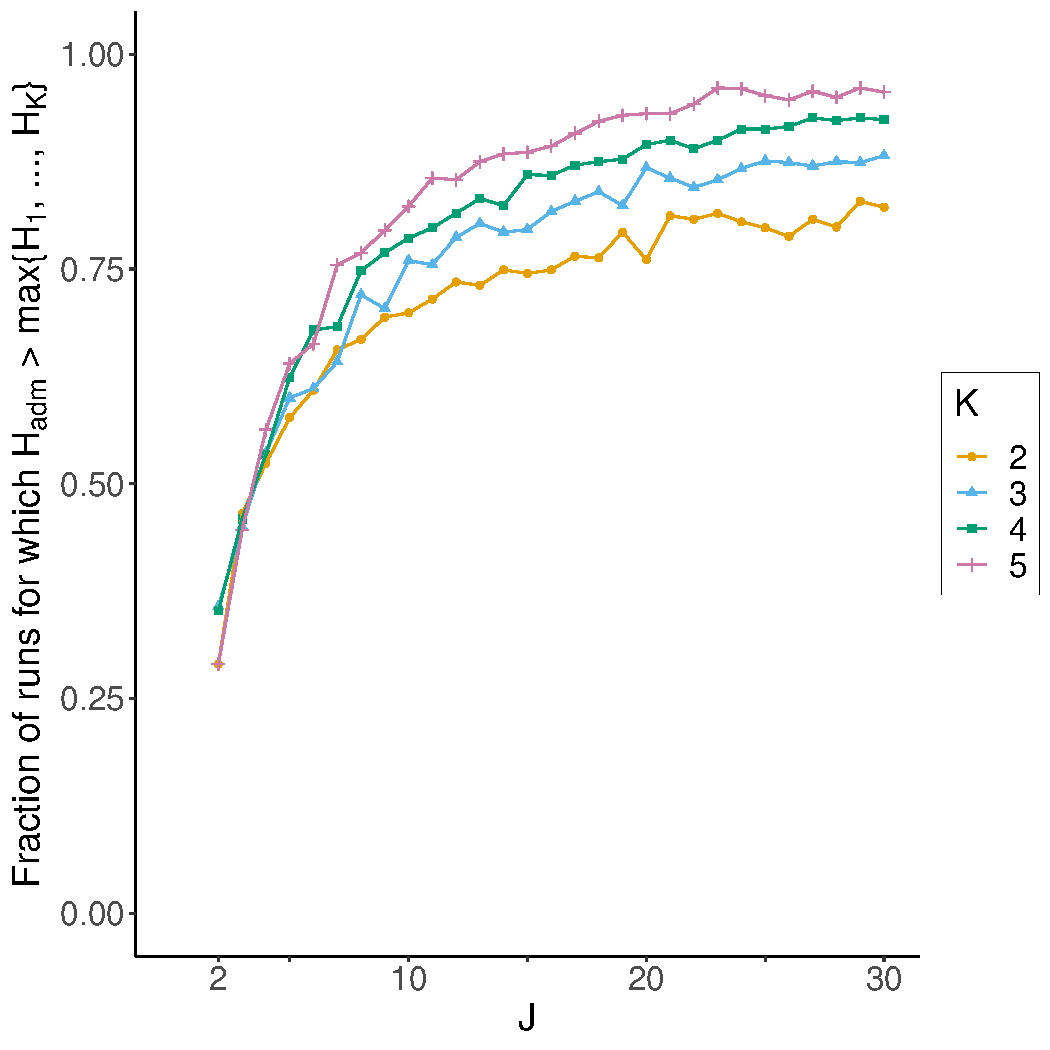
\includegraphics[width=\maxwidth]{../figs/Fig4-1} 

\end{knitrout}
